
\newpage
\begin{center}
\textbf{\large ГЛАВА 3 \\ Диффузия на жидких бинодальях: влияние дальнодействия силы притяжения}
\end{center}
\refstepcounter{chapter}

\addcontentsline{toc}{chapter}{ГЛАВА 3. Диффузия на жидких бинодальях: влияние дальнодействия силы притяжения}

В данной работе используется моделирование молекулярной динамики для расчета фазовых диаграмм обобщенных систем Леннарда-Джонса с различными показателями притяжения. Оценены коэффициенты диффузии и подвижности (обратной диффузии) и проанализированы спектры коллективного возбуждения на жидких бинодалиях. Отмечено, что зависимость коэффициента подвижности от температуры является линейной в широком диапазоне температур, а ее наклон увеличивается с увеличением показателя притяжения. В начале нелинейной зависимости подвижности от температуры дисперсионные соотношения коллективных возбуждений жидкости обнаруживают переход от колебательного к монотонному ходу.

\section{Роль диффузии в науке и технике}
\label{MACR-SecIntroduction}

Диффузия играет важную роль в различных процессах переноса массы, начиная от науки и техники и заканчивая живой природой.
Он играет решающую роль в биологических процессах~\cite{10.1016/j.bbagen.2013.09.037, 10.1038/s41598-018-22643-9}, а также в механизмах и кинетике химических реакций. Знание механизмов диффузии позволит добиться значительного прогресса в новых биотехнологиях и медицине, решить важные проблемы химической и фармакологической промышленности и не только~\cite{10.1002/3527602836}.

Процесс диффузии очень хорошо изучен в газах и твердых телах. Например, очень подробное знание процесса диффузии достигается в кристаллических системах~\cite{10.1016/0079-6816(95)00039-2} из-за его практической важности в металлургии для легирования~\cite{10.1016/s0924-0136(96)02826-9, 10.1016/j.actamat.2015.10.010, 10.1134/s1063783411110308} и эксплуатации полупроводниковой электроники~\cite{10.1103/physrevlett.84.4220, 10.1016/j.physrep.2009.10.003}.

В этой главе, используя метод молекулярной динамики (МД), моделируются обобщенные системы Леннарда-Джонса с различными показателями притяжения. Рассчитаны температурные зависимости подвижности частиц (коэффициента обратной диффузии) на бинодали жидкости. Основной целью главы является установление связи между диффузией, дальнодействием межчастичного притяжения и свойствами коллективных возбуждений в простых жидкостях.

\section{Методы}
\label{MACR-SecMethods}

\subsection{Расчет фазовых диаграмм методами молекулярной динамики}
\label{MACR-SubSecMD}

В данной главе анализируются транспортные свойства и их связь с коллективными модами на жидких бинодальях.
для систем, взаимодействующих через обобщенный потенциал Леннарда-Джонса (LJ$n$-$m$):
\begin{equation}
U_{n-m}(r)=4 \varepsilon\left[\left(\frac{\sigma}{r}\right)^{n}-\left(\frac{\sigma}{r}\right)^{m}\right]
\label{MACR-eq1}
\end{equation}
где $\epsilon$ и $\sigma$ — характерные масштабы энергии и длины соответственно. На протяжении всей статьи используются приведенные единицы измерения температуры $ T/ \epsilon \rightarrow T $, расстояния $ r/ \sigma \rightarrow r $ и плотности $ \rho \sigma ^ 3 \rightarrow n$.


Были рассмотрены потенциалы LJ$12$-$4$, LJ$12$-$5$, LJ$12$-$6$ и LJ$16$-$6$. Были также смоделировали этан~\cite{10.1021/acs.jced.6b01036}, чтобы сравнить полученные результаты для LJ$n$-$m$ с результатами для системы, в которой взаимодействия не являются сферически-симметричными.
В выбранной модели молекула этана рассматривается как пара жестко связанных радикалов CH$_3$, взаимодействующих с радикалами других молекул через потенциал~\cite{10.1021/acs.jced.6b01036}:
\begin{equation}
U_{\rm {ethane}}(r) = \tilde \varepsilon\left[\left(\frac{\sigma}{r}\right)^{16}-\left(\frac{\sigma}{r}\right)^{6}\right],
\label{MACR-eq2}
\end{equation}
где $\tilde\varepsilon = 0,69396$ ккал/моль и $\sigma = 3,783$\AA.

Все МД-симуляции были выполнены в ансамбле NVT (N, V и T - количество частиц, объем системы и температура соответственно) с периодическими граничными условиями с использованием пакета моделирования LAMMPS~\cite{10.1006/jcph.1995.1039} .
На первом этапе были рассчитаны линии бинодали по ссылкам~\cite{10.1021/jp806127j, 10.1021/jp1117213}.
Исходное состояние системы формировалось в два этапа: (i) кубический ящик моделирования заполнялся равновесным кристаллом (в нашем случае ГЦК) из $N$ частиц с плотностью, соответствующей близкому к нулю давлению; (ii) окно моделирования было расширено в направлении осей $x$ так, чтобы окончательная средняя плотность системы $\rho_a$ стала равной значениям, указанным в таблице~\ref{MACR-Table1}.
Результирующее начальное состояние показано на рис.~\ref{MACR-Figure1}(а).
Затем температура системы линейно увеличивалась от $T_{start}$ до $T_{stop}$ в течение $n_{step}$ шагов моделирования с временным шагом $\Delta t$.
Конденсированная фаза в какой-то момент начинает испаряться, образуя сосуществование газа и конденсата, если температура ниже критической, как показано на рис.~\ref{MACR-Figure1}(b).
Принципиально то, что полученное таким образом состояние системы почти всегда имеет границы фаз, ортогональные оси $x$.
В результате плотности $\rho_g$ и $\rho_c$ газовой и конденсированной фаз соответственно могут быть рассчитаны путем подгонки профиля плотности $\rho(x)$ выражением~\cite{10.1021/jp806127j, 10.1021/jp1117213}:

\begin{equation}
    \rho(x)=\frac{\rho_{l}+\rho_{g}}{2}-\frac{\rho_{l}-\rho_{g}}{2} \tanh \left(\frac{|x|-L}{\delta}\right),
    \label{MACR-eq3}
\end{equation}
где $L$ — половина площади, занимаемой жидкой фазой, а $\delta$ — характерная ширина границы раздела.
Пример профиля плотности системы и его аппроксимация уравнением~\eqref{MACR-eq3} показаны на рис.~\ref{MACR-Figure1}(c) гистограммой и красной линией соответственно.
Параметры моделирования для рассмотренных моделей сведены в табл.~\ref{MACR-Table1}.

\begin{table}[]
\centering
\begin{tabular}{|lllllcl|}
\hline
\multicolumn{1}{|l|}{Potential} & \multicolumn{1}{l|}{$\rho_a$} & \multicolumn{1}{l|}{$r_c$} & \multicolumn{1}{l|}{$T_{start}$} & \multicolumn{1}{l|}{$T_{stop}$} & \multicolumn{1}{l|}{$n_{step}$}                       & $\Delta t$                          \\ \hline
\multicolumn{7}{|c|}{Значения в безразмерных единицах:}                                                                                                                                                                                                         \\ \hline
\multicolumn{1}{|l|}{LJ12-4}    & \multicolumn{1}{l|}{0.25}     & \multicolumn{1}{l|}{15.0}  & \multicolumn{1}{l|}{1.0}         & \multicolumn{1}{l|}{5.5}        & \multicolumn{1}{c|}{\multirow{4}{*}{$3 \times 10^6$}} & \multirow{4}{*}{$5 \times 10^{-4}$} \\ \cline{1-5}
\multicolumn{1}{|l|}{LJ12-5}    & \multicolumn{1}{l|}{0.25}     & \multicolumn{1}{l|}{10.0}  & \multicolumn{1}{l|}{0.8}         & \multicolumn{1}{l|}{2.4}        & \multicolumn{1}{c|}{}                                 &                                     \\ \cline{1-5}
\multicolumn{1}{|l|}{LJ12-6}    & \multicolumn{1}{l|}{0.35}     & \multicolumn{1}{l|}{8.0}   & \multicolumn{1}{l|}{0.5}         & \multicolumn{1}{l|}{1.4}        & \multicolumn{1}{c|}{}                                 &                                     \\ \cline{1-5}
\multicolumn{1}{|l|}{LJ16-6}    & \multicolumn{1}{l|}{0.31}     & \multicolumn{1}{l|}{8.0}   & \multicolumn{1}{l|}{0.8}         & \multicolumn{1}{l|}{1.6}        & \multicolumn{1}{c|}{}                                 &                                     \\ \hline
\multicolumn{7}{|c|}{Единицы измерения СИ:}                                                                                                                                                                                                                     \\ \hline
\multicolumn{1}{|l|}{Ethane}    & \multicolumn{1}{l|}{$0.22\mathrm{\frac{g}{cm^3}}$}     & \multicolumn{1}{l|}{$25\text{\AA}$}    & \multicolumn{1}{l|}{$80\,\mathrm{K}$}          & \multicolumn{1}{l|}{$320\,\mathrm{K}$}        & \multicolumn{1}{l|}{$2 \times 10^6$}                  & $2\,\mathrm{\text{фс}}$                                   \\ \hline
\end{tabular}
\caption{Параметры, используемые в МД-моделировании для бимодальных расчетов: где $\rho$ — средняя плотность системы, $r_c$ — радиус отсечки, $T_{start}$ и $T_{stop}$ — начальная и конечная температуры. моделирования, соответственно, $n_{step}$ — количество шагов моделирования, а $\Delta t$ — временной шаг.}
\label{MACR-Table1}
\end{table}


\begin{figure}[!t]
\centering
 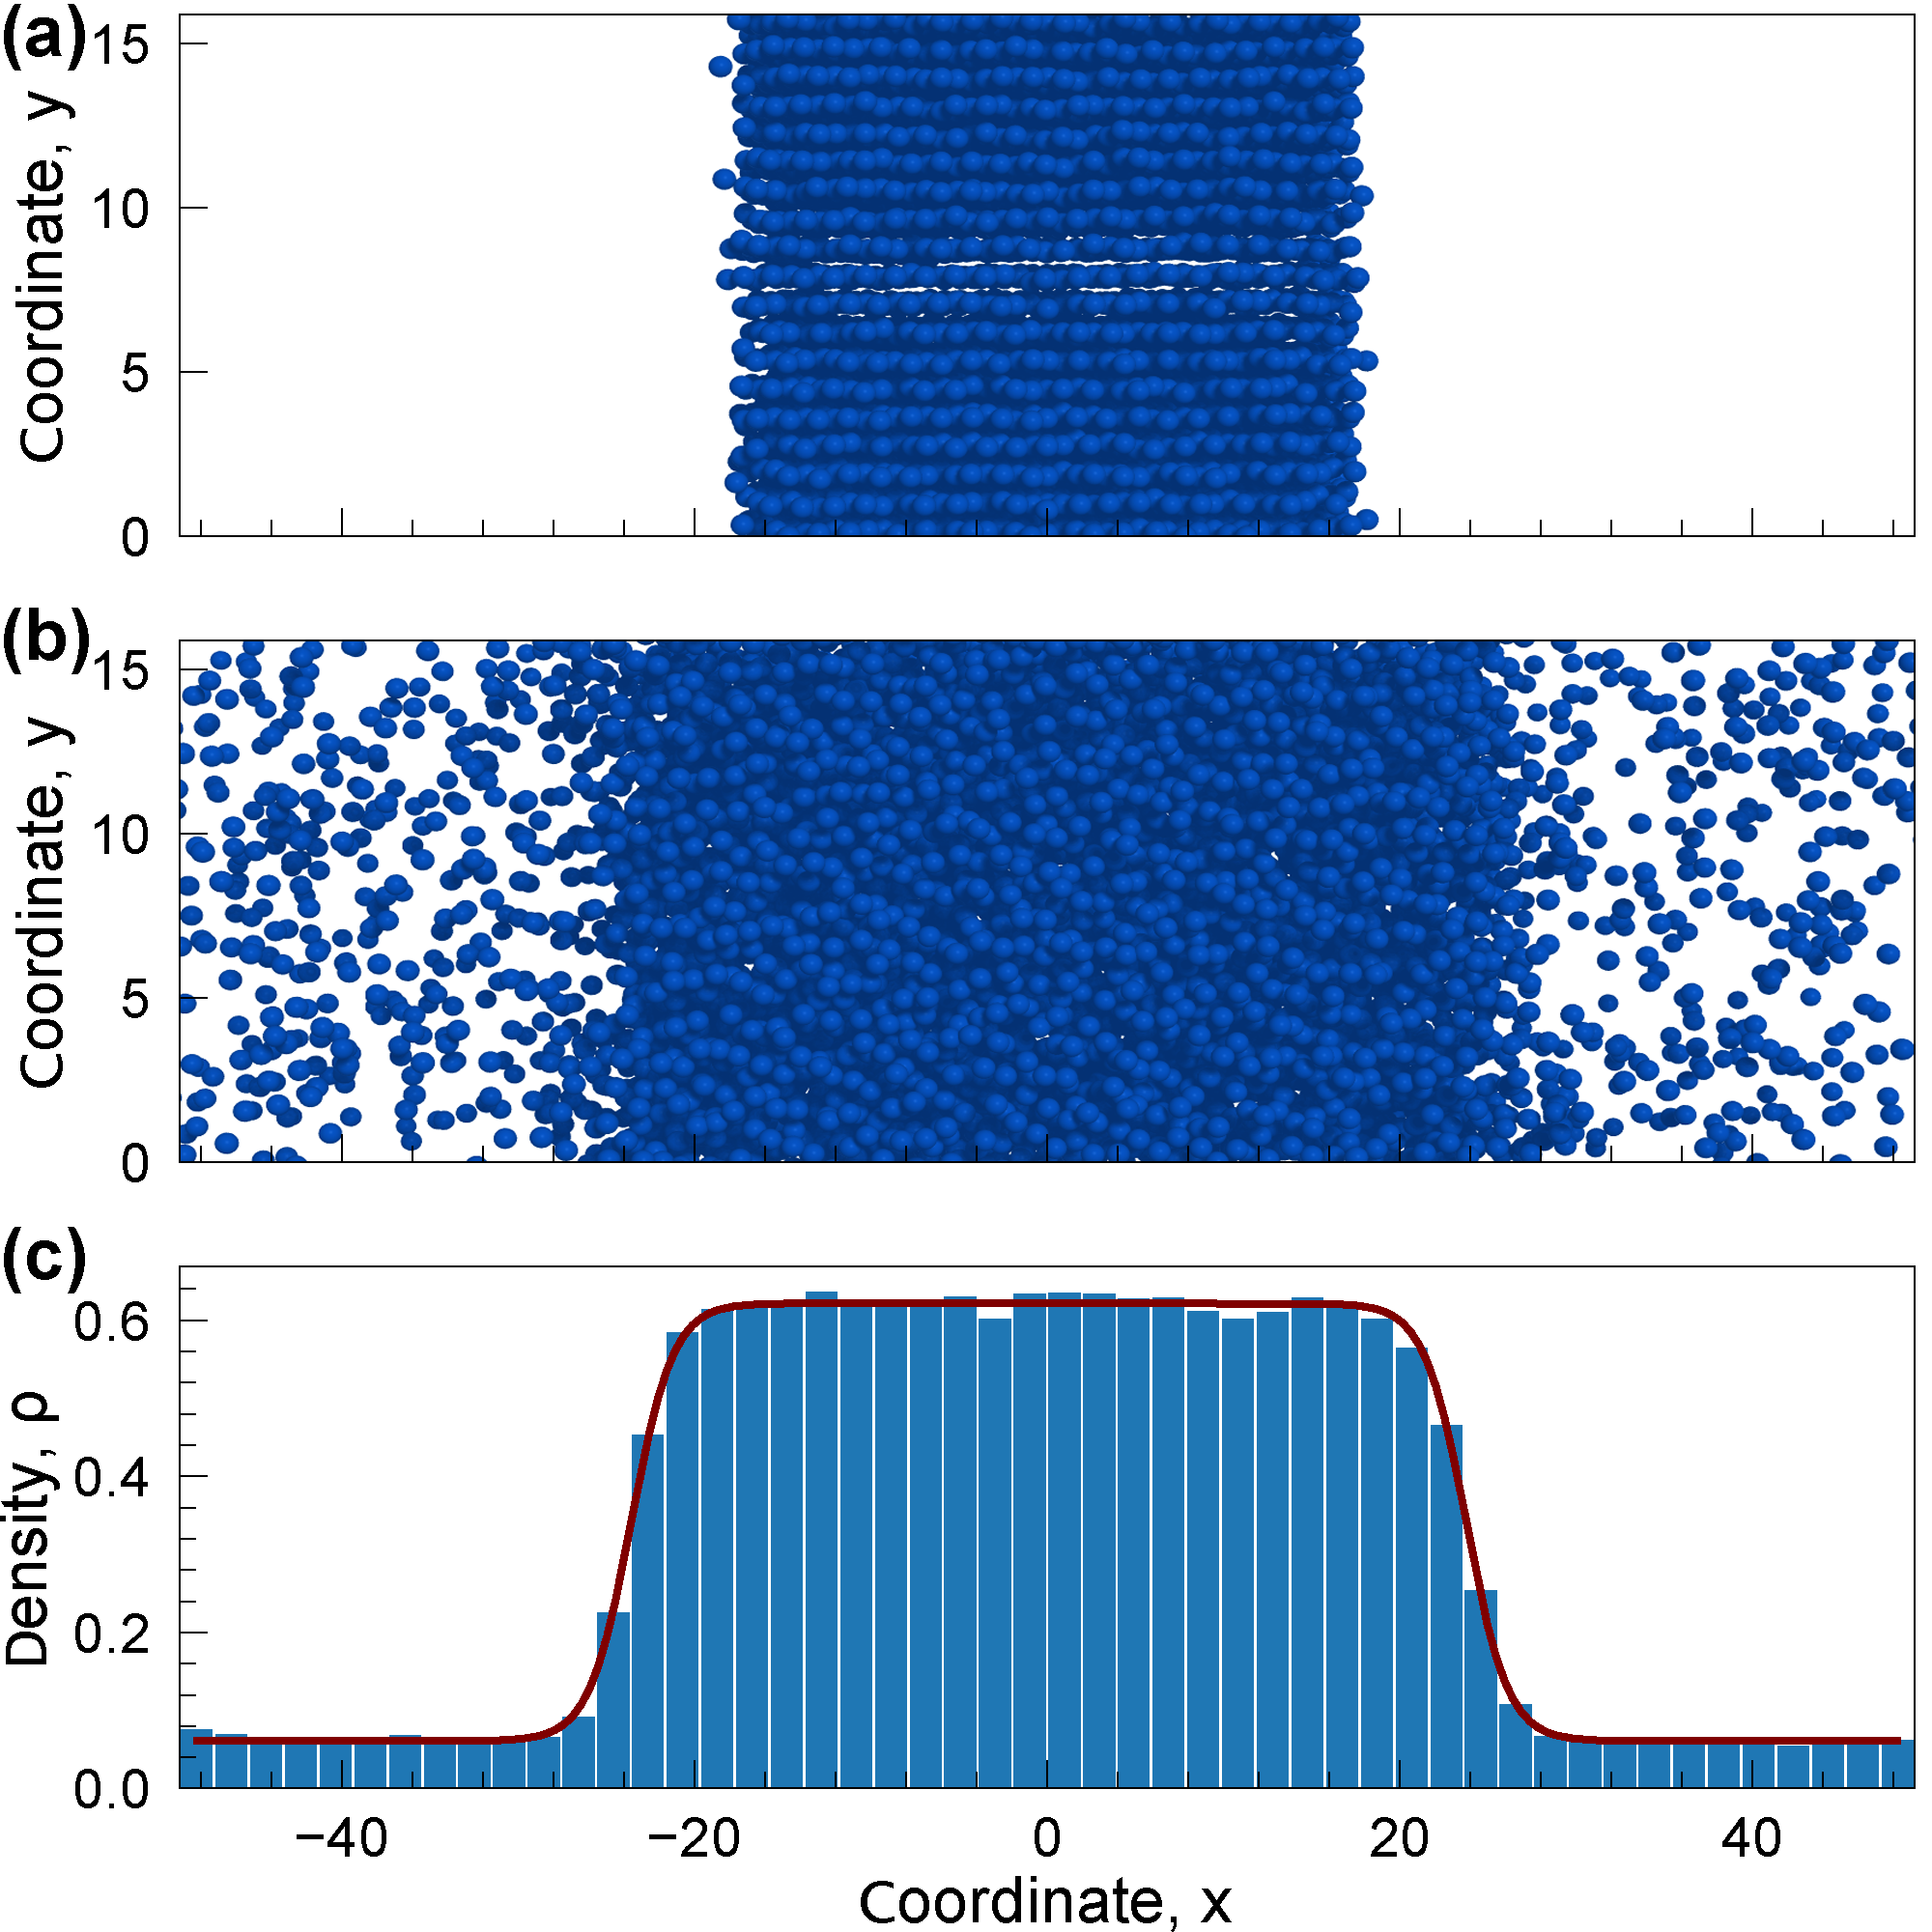
\includegraphics[width=85mm]{MACR-Figure1.png}
 \caption{(a) Система частиц для расчета фазовой диаграммы. Система частиц с потенциалом взаимодействия LJ12-6 при температуре $T=1.13$ в виде плоского слоя.
   (b) Профиль плотности системы вдоль оси $x$. Область с высокой плотностью представляет собой конденсат, с низкой - газ. Темно-красная линия представляет собой аппроксимацию профиля плотности уравнением~\eqref{MACR-eq3}.}
\label{MACR-Figure1}
\end{figure}


\begin{figure}[!t]
\centering
 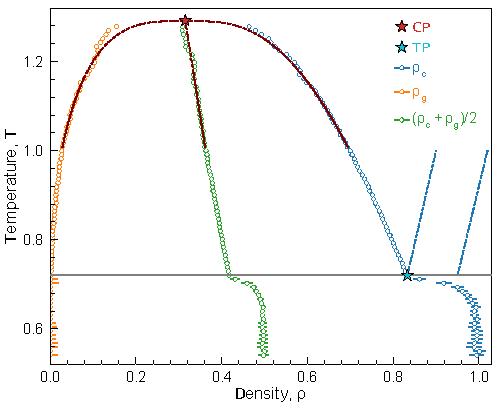
\includegraphics[width=85mm]{MACR-Figure2.pdf}
 \caption{Фазовая диаграмма системы LJ12-6.
  Оранжевые и синие символы — плотности газа и конденсата, полученные путем подгонки данных МД по уравнению~\eqref{MACR-eq3}.
  Зеленые символы — это медиана $\rho_m=(\rho_g+\rho_c)/2$.
  Сплошная красная линия соответствует уравнению~\eqref{MACR-eq4}.
  Тройные и критические точки обозначены синими и красными звездочками соответственно.
 }
\label{MACR-Figure2}
\end{figure}

Вблизи критической температуры расчет плотности газа и жидкости становится затруднительным из-за усиленных флуктуаций плотности.
Однако положение критической точки на фазовой диаграмме можно вычислить, аппроксимируя жидкостную и газообразную бинодальные ветви вблизи критической точки выражением:
\begin{equation}
    \rho_{l}-\rho_{g} \simeq A \tau^{\beta}, \quad \rho_{l}+\rho_{g} \simeq a \tau+2 \rho_{\mathrm{CP}},
\label{MACR-eq4}
\end{equation}

где $\tau=T_{\mathrm{CP}}-T$, $T_{\mathrm{CP}}$ и $\rho_{\mathrm{CP}}$ - температура и плотность в критической точке, $ \beta$ — критический индекс, $A$ и $a$ — свободные параметры.
Критический индекс $\beta$ зависит от класса универсальности системы, который определяется механизмами межчастичных взаимодействий~\cite{10.1103/physrevlett.89.025703}.
В трех пространственных измерениях критический индекс $\beta_c = 0,5$ для потенциала LJ$12-4$, тогда как $\beta_c = 0,325$ для LJ$12$-$5$, LJ$12$-$6$, LJ$16$-$6$ и этан, согласно предыдущим результатам~\cite{10.1021/acs.jced.6b01036,10.1021/jp9072137,10.1103/physrevlett.89.025703}.

Пример полученных бинодалей для LJ12-6 и их околокритическая аппроксимация уравнением~\eqref{MACR-eq4} показаны на рис.~\ref{MACR-Figure2}.
Обратите внимание, что на конденсированной бинодали имеется явный излом (см. рис.~\ref{MACR-Figure2}), который указывает на падение плотности при плавлении и соответствует положению тройной точки.
Полученные значения $A$ и $a$ аппроксимационного уравнения~\eqref{MACR-eq4}, а также плотности и температуры критических и тройных точек для рассматриваемых систем сведены в табл.~\ref{MACR-Table2}.

\begin{figure}[!t]
\centering
 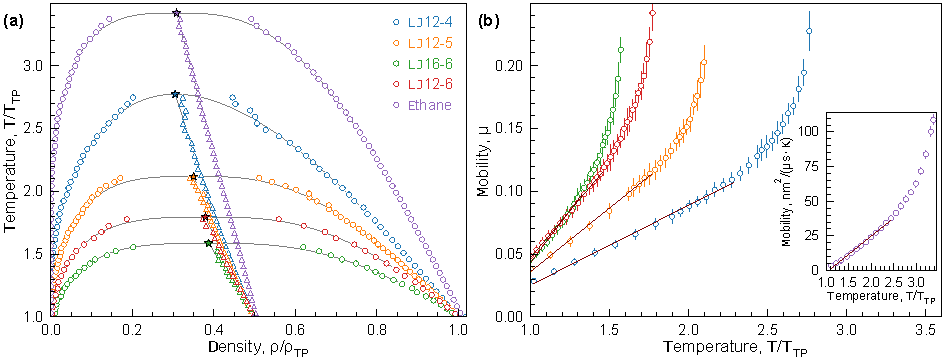
\includegraphics[width=170mm]{MACR-Figure3.pdf}
 \caption{(а) Фазовые диаграммы рассматриваемых систем. Фазовые диаграммы рассчитывались методом двухфазного моделирования, описанным в разделе~\ref{MACR-SecMethods}. Цветные точки обозначают рассчитанные бинодали, треугольники обозначают срединные точки. Сплошные серые кривые показывают диапазон температур, используемый для аппроксимации и определения параметров в уравнении ~\eqref{MACR-eq4}. Штриховые серые кривые соответствуют экстраполированным биноидам. (б) Температурная зависимость подвижности частиц. Подвижность частиц была рассчитана на жидких бинодальях с использованием метода, описанного в разделе~\ref{MACR-SecMethods}. Точки, соответствующие экстраполированным бинодалим, отмечены серым цветом. Прямые линии соответствуют линейной аппроксимации подвижности. На вставке показана расчетная подвижность метана.}
\label{MACR-Figure3}
\end{figure}

\subsection{Расчет диффузии и спектров на конденсированной бинодали}

Далее для расчета подвижности на конденсированной бинодали моделировались системы с плотностью и температурой, взятыми из полученных фазовых диаграмм.
Для обобщенных леннард-джонсовских систем с $N = 4,0 \times 10 ^ 3$ моделировались шаги по времени $1,5 \times 10 ^ 5$. Для этана использовались $N = 1,065 \times 10 ^ 4 $ молекул и проведены моделирования с временными шагами $ 7,0 \times 10 ^ 5 $. Для релаксации системы использовались первые шаги по времени $ 5,0 \times 10 ^ 4 $ для обобщенных LJ-систем и шаги $ 5,0 \times 10 ^ 5 $ для этана. Остальные параметры были такими же, как и при расчете фазовых диаграмм.

Коэффициент самодиффузии $D$ определялся по среднеквадратичному отклонению частиц:
\begin{equation}
    \sigma^2(t) = \sum\limits_{\alpha = 1}^{N} (r_{\alpha}(t) - r_{\alpha}(0))^2 / N, \quad \sigma^2(t) = 6Dt,
    \label{MACR-eq5}
\end{equation}
где $\sigma$ — среднеквадратичное отклонение, а $t$ — время. Подвижность $\mu$ связана с коэффициентом диффузии соотношением Эйнштейна
\begin{equation}
    \mu = \frac{D}{T},
    \label{MACR-eq6}
\end{equation}
где $T$ — температура системы.

Наконец, спектры возбуждения были получены с использованием обработки тока скорости~\cite{10.1063/1.5050708}:
\begin{equation}
    C_{L, T}(\mathbf{q}, \omega)=\int dt e^{i \omega t} \text{Re} \left\langle\mathbf{j}_{L, T}(\mathbf{q}, t) \mathbf{j}_{L, T}(-\mathbf{q}, 0)\right\rangle,
    \label{MACR-eq7}
\end{equation}
где ${\bf k}$ и $\omega$ — волновой вектор и частота,
$\mathbf{j}_{L}=\mathbf{q}(\mathbf{j} \cdot \mathbf{q} ) / q^{2}$ и $\mathbf{j}_{T}=(\mathbf{j \cdot e_{\perp})e_{\perp}}$ — продольная ($L$) и поперечная ($T$) компоненты тока частиц,\\
$\mathbf{j}(\mathbf{q}, t)=N^{-1} \sum_{s} \mathbf{v}_{s}(t) \ exp \left(i \mathbf{q} \mathbf{r}_{s}(t)\right)$ и $\mathbf{v}_{s}(t)=\dot{\mathbf{r} }_{s}(t)$ — скорость $s$-й частицы.
Суммирование ведется по всем $N$ частицам в системе. Усреднение по каноническому ансамблю обозначается $\langle\cdots\rangle$. Анализ $C_{L, T}(\mathbf{q}, \omega)$ проводился по методикам, описанным в~\cite{10.1038/s41598-019-46979-y}, что позволило получить дисперсионные соотношения продольной и поперечной мод.

МД-моделирование для расчета спектров возбуждения отличается от моделирования для подвижности только длительностью временного шага. Для LJ$12$-$4$ и LJ$16$-$6$ шаг по времени был выбран как $\Delta t = 1 \times 10 ^ {-4} \sqrt {m \sigma ^ 2 / \epsilon}$, а для LJ$12$-$5$ и LJ$12$-$6$ шаг по времени составлял $\Delta t = 5 \times 10 ^ {-4} \sqrt {m \sigma ^ 2 / \epsilon}$.

\begin{figure}[!t]
\centering
 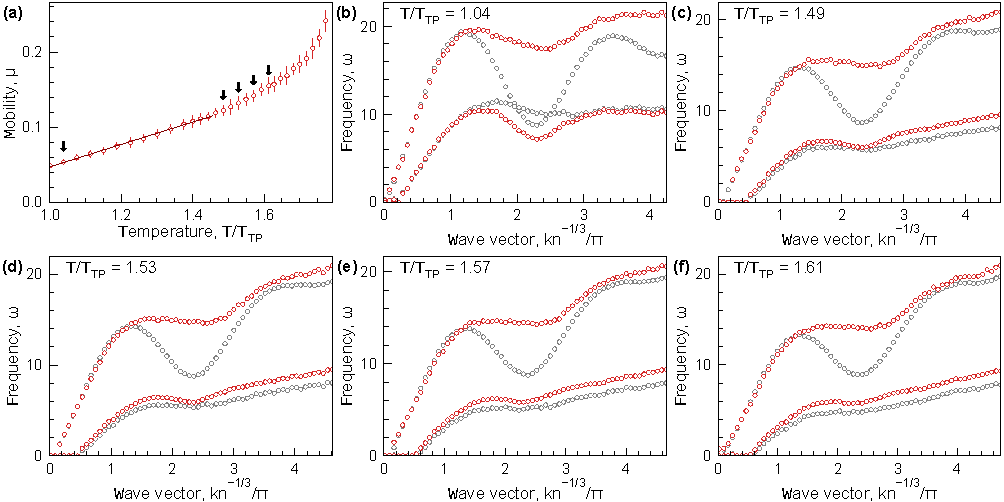
\includegraphics[width=170mm]{MACR-Figure4.pdf}
 \caption{(a) Температурная зависимость подвижности системы LJ$12$-$6$ вдоль жидкостной бинодали.
  Температуры, при которых рассчитывались спектры возбуждения, указаны черными стрелками.
  (b) - (f) спектры возбуждения LJ$12$-$6$ систем.
Спектры рассчитывались путем анализа скорости течения (уравнение~\eqref{MACR-eq7}) так же, как в Ref.~\cite{10.1038/s41598-019-46979-y}.
  Красный цвет соответствует гибридным модам, серый — результатам анализа отдельных мод~\cite{10.1038/s41598-019-46979-y}.
  В левом верхнем углу указаны пониженные температуры.}
\label{MACR-Figure4}
\end{figure}

\section{Результаты}
\label{MACR-SecResults}

Результаты расчета границ сосуществования газа и жидкости показаны на рис.~\ref{MACR-Figure3}(а).
Цветные точки обозначают бинодали, треугольники соответствуют срединным точкам.
Точки, которые использовались для аппроксимации [с использованием уравнения~(\ref{MACR-eq4})], выделены сплошной серой линией.
Экстраполированные бинодали обозначены пунктирной серой линией.
Для каждой рассматриваемой системы температура и плотность выражаются в единицах температуры и плотности тройной точки соответственно.
Последние значения вместе с параметрами критических точек приведены в Таб.~\ref{MACR-Table2}.

\begin{table}[h!]
    \centering{
    \begin{tabular}{C{1.5cm}|C{1.0cm}|C{1.0cm}|C{1.0cm}|C{1.0cm}|C{1.0cm}|C{1.0cm}}
        LJn-m & $T_{\rm CP}$ & $\rho_{\rm CP}$ & $T_{\rm TP}$ & $\rho_{\rm TP}$ & $A$ & $a$ \\ \hline
        LJ12-4 & 4.85 & 0.291 & 1.75 & 0.952 & 0.559 & 0.107 \\
        LJ12-5 & 2.18 & 0.304 & 1.03 & 0.867 & 0.804 & 0.208 \\
        LJ12-6 & 1.29 & 0.315 & 0.72 & 0.830 & 1.002 & 0.326 \\
        LJ16-6 & 1.55 & 0.316 & 0.98 & 0.816 & 0.969 & 0.334 \\
        Ethane & 305.3 & 206.7 & 90.34 & 651.9 & 113.1 & 1.158
    \end{tabular}

    }
    \caption{Значения плотностей и температур критических и тройных точек и параметры аппроксимации по уравнению~\eqref{MACR-eq4} для рассматриваемых моделей.
     Для обобщенных систем LJ температуры и плотности даны в сокращенных единицах. Для этана температура выражена в К, а плотность выражена в $\text{кг}/\text{м}^3$. Параметры критической и тройной точек для этана взяты из работы~\cite{10.1063/1.555785}.}
    \label{MACR-Table2}
\end{table}

Замечено, что с увеличением дальнодействующего характера потенциала температуры тройной и критической точек, а также их отношение $T_{\rm CP}/T_{\rm TP}$ также увеличивать.

Затем по рассчитанным фазовым диаграммам рассчитывали подвижность частиц при плотностях и температурах, соответствующих бинодали жидкости. Полученная зависимость подвижности частиц от температуры представлена на рис.~\ref{MACR-Figure3}(b). Цветные точки на (b) соответствуют цветным точкам на (a). Серые точки обозначают подвижности на экстраполированных частях бинодали.

Заметим, что при низких температурах подвижность на бинодали имеет линейную зависимость от температуры. Его наклон увеличивается с уменьшением дальнодействующего характера потенциала взаимодействия (т. е. с увеличением показателя притяжения). Линейная зависимость сохраняется до определенной температуры, а затем становится нелинейной. Возникновение такой нелинейности может быть связано с особенностями коллективной динамики частиц, которые должны коррелировать со спектрами коллективных возбуждений.

Расчетные спектры системы LJ$12$-$6$ показаны на рис.~\ref{MACR-Figure4}. На рис.~\ref{MACR-Figure4}(а) показана зависимость подвижности от температуры, а черными стрелками указаны температуры, при которых рассчитывались спектры. Были выбраны несколько точек вблизи температуры, при которой наблюдается начало нелинейной зависимости, и одну температуру вблизи тройной точки. На рис.~\ref{MACR-Figure4}(b)-(f) показаны расчетные соотношения дисперсии продольных и поперечных мод в этих точках. Красный цвет соответствует модели с двумя осцилляторами, а серый — одномодовому анализу~\cite{10.1038/s41598-019-46979-y}.

Нетрудно заметить, что по мере приближения температуры к точке, соответствующей возникновению нелинейной зависимости, дисперсионные соотношения демонстрируют переход от осциллирующей к монотонной зависимости от волнового числа. Таким образом, качественное изменение температурной зависимости подвижности частиц сопровождается количественным изменением спектров возбуждения. Наблюдаемая картина не является специфической для системы LJ$12$-$6$. Аналогичная тенденция наблюдается и для других исследованных обобщенных ЛД-систем (спектры их коллективных возбуждений см. в Приложении). Это дает новое свидетельство тесной связи между переносом жидкости и свойствами коллективного возбуждения.

\section{Заключение главы}
\label{MACR-SecConclusions}

В настоящей работе исследовано влияние формы потенциала парного взаимодействия на фазовые диаграммы и подвижность частиц в жидкой фазе. Были рассчитаны кривые сосуществования газа и жидкости для потенциалов с переменной относительной силой притяжения. Было замечено, что с увеличением дальнодействующего характера потенциала температуры тройной и критической точек, а также их отношение $T_{\rm CP}/T_{\rm TP}$ также увеличивать. Коэффициент диффузии и обратный ему коэффициент подвижности вычислялись на жидких бинодалиях. Обнаружено, что температурная зависимость подвижности линейна в широком диапазоне температур с тем большим наклоном, чем меньше диапазон притяжения. Кроме того, установлено, что начало нелинейной температурной зависимости подвижности при высоких температурах совпадает с переходом дисперсионных зависимостей коллективных возбуждений от осциллирующей к монотонной зависимости от волнового числа. Эти результаты открывают возможности для дальнейшего изучения диффузии и ее связи с коллективными процессами в конденсированных многочастичных системах.


\begin{figure}
\centering
 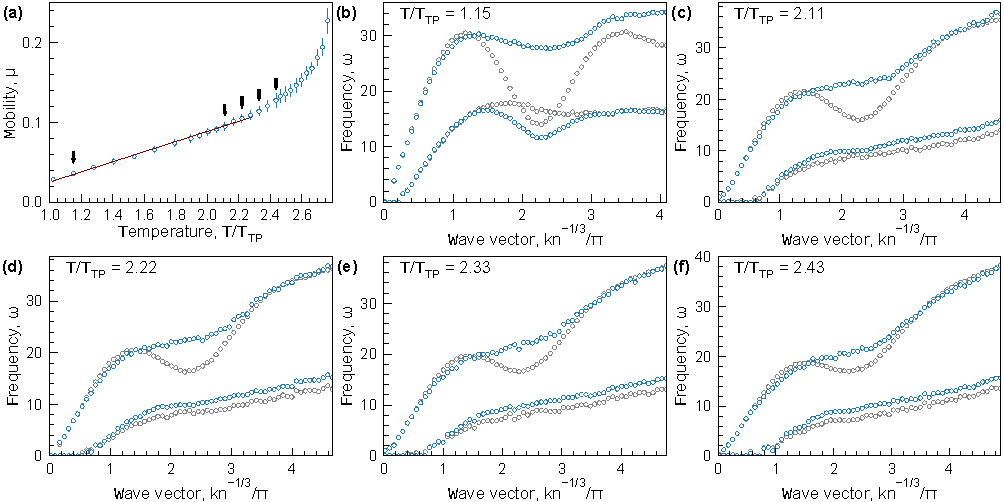
\includegraphics[width=150mm]{MACR-Figure5.pdf}
 \caption{Результаты для потенциала LJ$12$-$4$. Рисунок аналогичен рисунку~\ref{MACR-Figure4}(a)-(f).}
\label{MACR-Figure5}
\end{figure}


\begin{figure}
\centering
 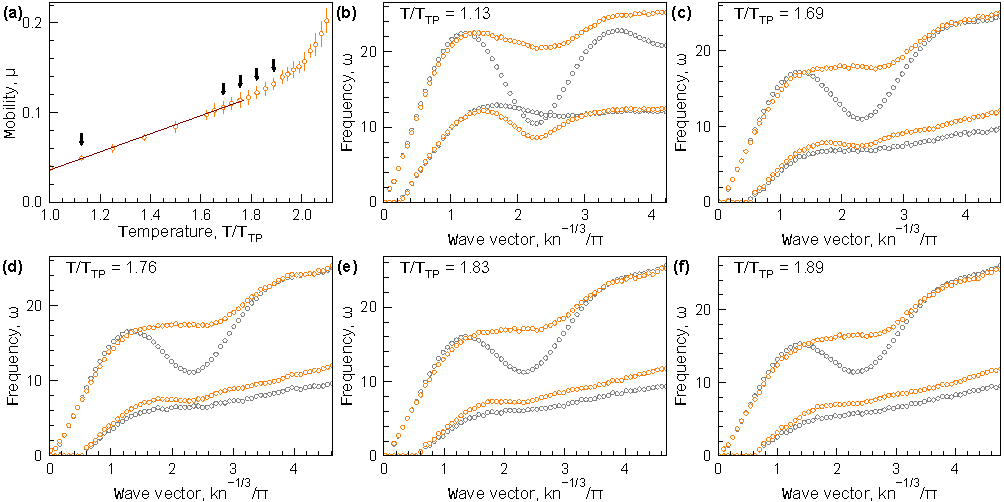
\includegraphics[width=150mm]{MACR-Figure6.pdf}
 \caption{Результаты для потенциала LJ$12$-$5$. Рисунок аналогичен рисунку~\ref{MACR-Figure4}(a)-(f).}
\label{MACR-Figure6}
\end{figure}


\begin{figure}
\centering
 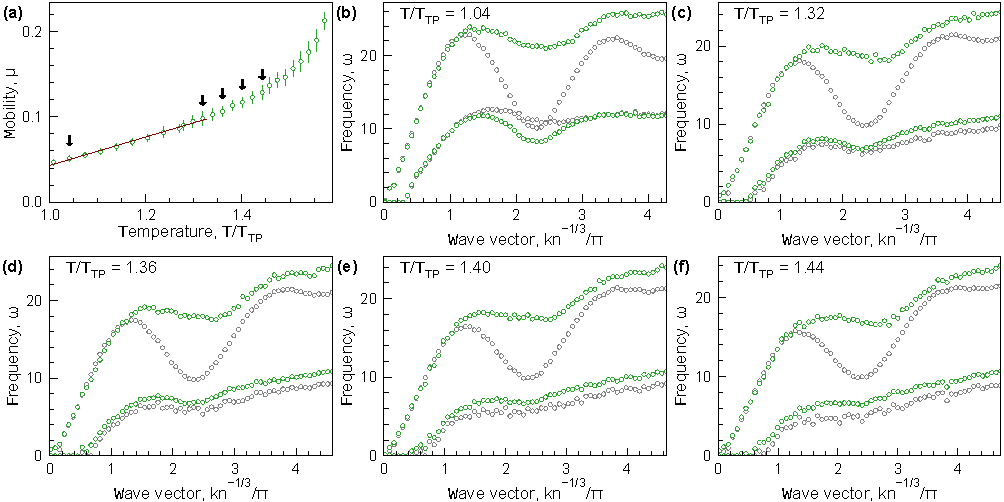
\includegraphics[width=150mm]{MACR-Figure7.pdf}
 \caption{Результаты для потенциала LJ$16$-$6$. Рисунок аналогичен рисунку~\ref{MACR-Figure4}(a)-(f).}
\label{MACR-Figure7}
\end{figure}
